%%%%%%%%%%%%%%%%%%%%%%%%%%%%%%%%%%%%%%%%%
% Short Sectioned Assignment
% LaTeX Template
% Version 1.0 (5/5/12)
%
% This template has been downloaded from:
% http://www.LaTeXTemplates.com
%
% Original author:
% Frits Wenneker (http://www.howtotex.com)
%
% License:
% CC BY-NC-SA 3.0 (http://creativecommons.org/licenses/by-nc-sa/3.0/)
%
%%%%%%%%%%%%%%%%%%%%%%%%%%%%%%%%%%%%%%%%%

%----------------------------------------------------------------------------------------
%	PACKAGES AND OTHER DOCUMENT CONFIGURATIONS
%----------------------------------------------------------------------------------------

\documentclass[paper=a4, fontsize=11pt]{scrartcl} % A4 paper and 11pt font size

\usepackage[T1]{fontenc} % Use 8-bit encoding that has 256 glyphs
\usepackage{fourier} % Use the Adobe Utopia font for the document - comment this line to return to the LaTeX default
\usepackage[english]{babel} % English language/hyphenation
\usepackage{amsmath,amsfonts,amsthm} % Math packages

\usepackage{lipsum} % Used for inserting dummy 'Lorem ipsum' text into the template

\usepackage{sectsty} % Allows customizing section commands
\allsectionsfont{\centering \normalfont\scshape} % Make all sections centered, the default font and small caps

\usepackage{fancyhdr} % Custom headers and footers
\pagestyle{fancyplain} % Makes all pages in the document conform to the custom headers and footers
\fancyhead{} % No page header - if you want one, create it in the same way as the footers below
\fancyfoot[L]{} % Empty left footer
\fancyfoot[C]{} % Empty center footer
\fancyfoot[R]{\thepage} % Page numbering for right footer
\renewcommand{\headrulewidth}{0pt} % Remove header underlines
\renewcommand{\footrulewidth}{0pt} % Remove footer underlines
\setlength{\headheight}{13.6pt} % Customize the height of the header

\numberwithin{equation}{section} % Number equations within sections (i.e. 1.1, 1.2, 2.1, 2.2 instead of 1, 2, 3, 4)
\numberwithin{figure}{section} % Number figures within sections (i.e. 1.1, 1.2, 2.1, 2.2 instead of 1, 2, 3, 4)
\numberwithin{table}{section} % Number tables within sections (i.e. 1.1, 1.2, 2.1, 2.2 instead of 1, 2, 3, 4)

%\setlength\parindent{5pt} % Removes all indentation from paragraphs - comment this line for an assignment with lots of text

%----------------------------------------------------------------------------------------
%			ADDED PACKAGES, ETC.
%----------------------------------------------------------------------------------------
\usepackage{setspace} % Allows for double spacing, etc.
\usepackage{hyperref} % links within document
\hypersetup{
    colorlinks=true,
    linkcolor=blue,
    filecolor=magenta,      
    urlcolor=cyan,
}

\usepackage{graphicx}% allows figures
\graphicspath{ {./images/} } 
\usepackage[margin=1in]{geometry}
\usepackage{bm} % allows bold

\DeclareMathOperator{\EX}{\mathbb{E}}% expected value
 
%----------------------------------------------------------------------------------------
%				GLOSSARY
%----------------------------------------------------------------------------------------
% Type these commands at the command line after editing glossary:
% pdflatex summary
% makeglossaries summary
% pdflatex summary

\usepackage{glossaries}
\makeglossaries
\loadglsentries{glossary}
\glsaddall % makes sure all definitions are in glossary even if they aren't mentioned in text

%----------------------------------------------------------------------------------------
%	TITLE SECTION
%----------------------------------------------------------------------------------------

\newcommand{\horrule}[1]{\rule{\linewidth}{#1}} % Create horizontal rule command with 1 argument of height

\title{	
\normalfont \normalsize 
\horrule{0.5pt} \\[0.4cm] % Thin top horizontal rule
\huge Data Science Toolkit \\ % The assignment title
\horrule{2pt} \\[0.5cm] % Thick bottom horizontal rule
}

\author{Matt Goodwin} % Your name

\date{\normalsize\today} % Today's date or a custom date
\onehalfspacing


%----------------------------------------------------------------------------------------
%	BEGIN DOCUMENT
%----------------------------------------------------------------------------------------

\begin{document}

% Print the title
\maketitle 

% Table of Contents
\tableofcontents
\newpage

%----------------------------------------------------------------------------------------
%	SECTION 1
%----------------------------------------------------------------------------------------

\section{Statistical Modeling}
\subsection{Overview and Theory}

When discussing modeling it is important to keep in mind that ``all models are wrong but some are useful'' \footnote{attributed to George Box}. The world is extremely complex and it can be impossible to create a model that perfectly approximates the underlying mechanisms that make our world turn.

There are different approaches to modeling depending on the discipline you come from, but personally I like the idea of the function approximation approach suggested by applied math and statistics. Taking this approach allows us to use probability theory combined with decision theory and to be able to visualize these concepts in a euclidean geometric space.

Bishop, from his book Pattern Recognition, has a really nice overview of some of these concepts. The starting point I think for modeling starts with independent variable or covariate $X$ (which could be a vector - see \hyperref[sec:notation]{notation} section) and dependent variable $Y$ (also could be a vector). We want to know:

\begin{enumerate}
\item The nature of the relationship between the variables (inference). 
\item Given an independent variable, determine the dependent variable (prediction).
\end{enumerate}

Using probability we can completely summarize the relationship and the uncertainty between the two variables with the joint distribution $P(X,Y)$. We use probability because for many problems we are interested in, we generally cannot come to a completely deterministic relationship between the independent and dependent variables. This is partly because of measurement error, but also because the number of independent variables needed to perfectly determine the dependent variable is potentially infinite. 

For example, imagine we wanted to predict the number of ice cream cones we will sell on a particular day. Some variables such as the time of year or location of the ice cream store may provide us enough information to make a pretty good prediction or to understand the relationship between the independent and dependent variables fairly well. But to perfectly predict the number of ice cream cones we would need to know everything from the state of the road conditions, to whether or not a family from out-of-state decided to take a vacation. Since this is impossible, we acknowledge variability and error in our estimates using probability.

I think the key to understanding this is to remember that the moment we use only a subset of all the possible features we would need for a perfectly deterministic relationship, then we must introduce uncertainty. We cannot say for certain that only knowing today is July 1 will lead to high ice-cream sales, but we can say the probability is higher than January 1st. When I have a training sample $(x_1, y_1), (x_2, y_2), ... (x_n, y_n)$,  I treat this as the truth (which it is) but I need to remember that these are draws coming from a distribution. I guess in that sense $P(X,Y)$ is a model itself, something we are forced to use because we don't know all the features needed for a deterministic relationship. 

One side note to make here is, as ESLII mentions, sometimes the relationship IS deterministic but the randomness comes from the fact that we have limited data. If we had a different training data set then we could get different results but the underlying relationship is deterministic. These problems can be handled by techniques appropriate for the error-based models described previously (see pg 28 of ESLII).

\subsubsection{Decision Theory}
As mentioned, we may want to perform inference, or in other words understand what $P(X,Y)$ looks like using information from a sample.  This can give us an understanding of how the variables are related. In many practical applications however, we want to be able to predict $Y$ given $X$. This is where decision theory comes into play. Decision theory is designed to help us make the optimal decision given inputs. Bishop gives a nice overview that I try and summarize in my own words below.

Lets approach this by treating the dependent variable $Y$ as a categorical variable taking on values 0 or 1. For simplicity assume $X$ is a single continuous variable. We then have for $P(X,Y)$ a three-dimensional distribution where $P(Y|X)$ is a probability mass function. When making a decision called the \emph{decision step} we formulate some rule that divides the input space into \emph{decision regions}. If an instance falls into a certain decision region (based on $X$) it is predicted to be a 0 or 1. We want to minimize our mistakes as much as possible so we aren't assigning an instance to 0 when it should really be 1. The probability of a mistake can be written as:

\begin{equation}
P(mistake) = P(X\in R_1, 0) + P(X\in R_0, 1)
\end{equation}
where $R_1$ is the region where an instance is assigned a 1 and $R_0$ is the region where an instance is assigned a 0.

Back to our example. Instead of ice cream sales, treat $Y$ as a categorical variable where 1 is a ``good'' ice cream sales day and 0 is ``bad''.  If $x_1$ = ``July 1st'' is in $R_1$ we decide to assign it a 1, based on our decision rule. However, even though our model $P(X,Y)$ says that the probability of a high-selling day ($Y=1$) is high in this region, there is a still a chance that it is a low-selling day because again, we are using a probability distribution for a model since we don't have all of the features we need for a deterministic model. The probability of it being a low-selling day for all $X$ in $R_1$ is $P(X\in R_1, 0)$, which is a mistake.

 \begin{figure}[t] \label{fig:bishop_optimal_distributions}
\caption{Plot from Bishop showing visually the optimal decision boundary}
\centering
 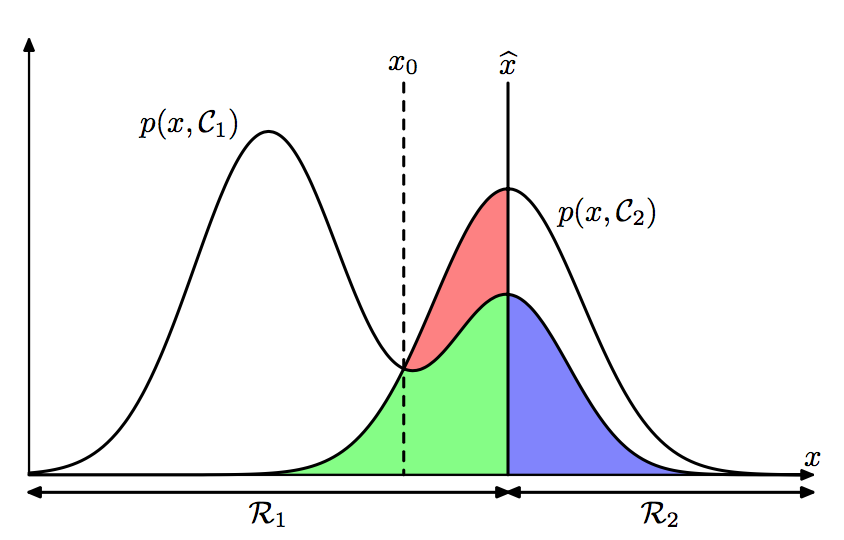
\includegraphics[scale=.7]{bishop_optimal_distributions.png}
 \end{figure}
 
We want to minimize our mistakes as much as possible so we choose regions where $P(X\in R_1, 0) + P(X\in R_0, 1)$ is as small as possible. To me it is easier to see this by thinking of the probability of being correct instead of the probability of being incorrect. This changes the problem from one of minimization to one of maximization. The optimal decision boundary therefore is the location that creates $R_1$ and $R_0$ such that $P(X\in R_1, 1) >  P(X\in R_1, 0)$ everywhere in $R_1$ and $P(X\in R_0, 0) >  P(X\in R_0, 1)$ everywhere in $R_0$. If the decision boundary were shifted either way then we would loose out on area under the distribution of being correct. 

To visualize this better refer to figure \ref{fig:bishop_optimal_distributions} from Bishop. If our decision boundary were at $x_0$ then the probability of being correct would be the two humped distribution completely colored in. This is the largest the probability of being correct can be. If we went with $\hat{x}$ however, then we loose out on the red region for being correct, which is suboptimal. (I like to think of a three dimensional distribution here whereas Bishop has an image with two different distributions which would need to be normalized appropriately but the concept is the same).

 We can use the product rule to write:
 
 \begin{equation}
 \begin{split}
 P(X\in R_1, 1) >  P(X\in R_1, 0)  & \implies  P(1|X\in R_1) P(X \in R_1) > P(0|X\in R_1) P(X \in R_1) \\
 & \implies  P(1|X\in R_1) > P(0|X\in R_1) 
 \end{split}
 \end{equation}
 So the maximization problem is equivalent to choosing the higher conditional probability for each region. This rule is known as the \emph{Bayes classifier} and the error rate of the Bayes classifier is known as the \emph{Bayes rate}. The Bayes classifier is used as a benchmark in classification as it is the optimal solution to classification if the probability distributions are known.
 
\subsubsection{Expected Loss Function}
Imbedded in the above discussion describing how to find the optimal decision rule is a concept called the \emph{loss function}. This is a function that takes as input the true class and predicted class (resulting from the chosen decision rule) and outputs a value encoding the error of the prediction. In the above examples we assume that the loss function is outputting a 0 for each class predicted correctly and a 1 for each class predicted incorrectly, so in other words all classes are weighted the same in terms of misclassification (this is also known as the 0-1 loss function). In some applications however, such as medical diagnosis, we want to weight some classes higher than others when calculating misclassification. For example, when diagnosing cancer it is much better to predict someone who is healthy as having cancer than the other way around.

For classification we can think of this function as a matrix known as the \emph{loss matrix}, but in general we can think of it as taking in two variables - the true class and the predicted class:

\begin{equation}
L(G, \hat{G}(X)).
\end{equation}

One issue with using this measure however is that we don't know the true class $G$. We can choose some decision rule to get us $\hat{G}$, but since we are dealing with probability distributions we won't know for sure whether the true class is a high-sales ice cream day or a low-sales ice cream day for example. Instead of minimizing the loss function then, we can minimize its expectation or in other words minimize the average loss function weighted by the probabilities for $G$ and $X$.

\begin{equation}
\begin{split}
E[L(G, \hat{G}(X))] & = \iint_{G, X} {L(G, \hat{G}(X)) P(G, X) dG dX} \\
& = \int_{X} \sum_{k=1}^{K} {L(G_k, \hat{G}(X)) P(G_k|X) P(X) dX} \\
&= E_{X} \sum_{k=1}^{K} {L(G_k, \hat{G}(X)) P(G_k|X)}
\end{split}
\end{equation}
where $k=1,...K$ are all of the classes, in our example either 0 or 1. We want to find a classifier $\hat{G}(X)$ such that the expected loss is minimal. To do this we can minimize the inner quantity pointwise since this corresponds to the minimum of the entire quantity (the minimum of an average is the minimum of the separate quantities in the average). This leads us to write:

\begin{equation}
\hat{G(x)} = \text{argmin}_{g \in G} \sum_{k=1}^{K} {L(G_k, g) P(G_k|X)}
\end{equation}
If we are using the 0-1 loss function then we can simplify this to:

\begin{equation}
\hat{G(x)} = \text{argmin}_{g \in G} \left[1 - P(g|X=x) \right].
\end{equation}
This took some thought for me to understand why we could simplify down to this. I think the best way to see it is to remember that this is a function of $g$. If we have $K=3$ for example then we can write out for each possible value of $G_k$:

\begin{equation}
\begin{split}
g=G_1 & \implies P(G_2|X=x) + P(G_3|X=x) \implies 1-P(G_1|X=x)\\
g=G_2 & \implies P(G_1|X=x) + P(G_3|X=x) \implies 1-P(G_2|X=x)\\
g=G_3 & \implies P(G_1|X=x) + P(G_2|X=x) \implies 1-P(G_3|X=x)\\
\end{split}
\end{equation}
since our loss function is 0 when it is a true classification and 1 when it is a misclassification. Since we are minimizing, the best choice for $g$ is the one where $P(g|X=x)$ is the largest (for each $x$) which corresponds to the Bayes classifier. Thus, we have proven that under the 0-1 loss function, the optimal decision is the Bayes classifier as we found in our previous discussion. Note that this is optimal when we know the distribution which most times we don't.

When we look more closely at the expected loss function $E[L(G, \hat{G}(X))]$, implied in here is some decision that is made that is represented by $\hat{G}(X)$. Since this decision is typically made based off of some sample (training data) and that sample is considered random, then this implies that we are omitting or hiding a important random variable - the random variable representing the sampling process. To see this better we can write the expectation above in the form of two expectations. The first is known as the \emph{test error}, the \emph{generalization error}, or \emph{prediction error}, all according to ESLII:

\begin{equation}
E[L(G, \hat{G}(X))|T].
\end{equation}
The variable $T$ represents a training set that we use to make a decision rule $\hat{G}(X)$. The training set $T$ is fixed in this expectation and the expectation is over the entire distribution of $X$ and $G$. Essentially, this is measuring the expected loss on potential new data fed into a model that was built on a given training set $T$. It is measuring how well our model generalizes to the entire population based off a model built on $T$.

If we take an expectation over all training sets and everything that is random then we have the original expected loss talked about earlier:

\begin{equation}
\begin{split}
E_{T}[E[L(G, \hat{G(X)})|T]] &= E_{T}[E_{G,X}[L(G, \hat{G(X)})|T]] \\
&= E_{T}\left[\iint_{G, X} {L(G, \hat{G}(X)) P(G,X|T) dG dX}\right]\\
&= \iiint_{G, X, T} {L(G, \hat{G}(X)) P(G,X|T) P(T) dG dX dT} \\
&= \iiint_{G, X, T} {L(G, \hat{G}(X)) P(G,X,T) dG dX dT}\\
&= E_{G,X,T}[L(G, \hat{G}(X))]\\
&= E[L(G, \hat{G}(X))]
\end{split}
\end{equation}
ELSII calls this the \emph{expected test error} or \emph{expected prediction error}.\\

\noindent TODO: Show graphs of general loss functions - see Stanford machine learning cheat sheet \newline
TODO: I think the expected loss is also known as the Risk function \newline
TODO: Show the regression loss function formulation. Note that the conditional mean is the optimal decision under the least squares loss just like the Bayes classifier is under the 0-1 loss. These loss functions are nice theoretically but may not be realistic in practice \newline
TODO: Explore the idea that the conditional mean is optimal IF we know the distribution just like the Bayes Classifier is optimal IF we know the distribution. \newline
TODO: Explore the dimensionality issue

\subsubsection{Bias-Variance Tradeoff}

The bias-variance tradeoff refers to two sources of error when evaluating models - the bias and the variance. There is also a third source of error which we call the ``irreducible error''. 

As explained in \href{https://towardsdatascience.com/mse-and-bias-variance-decomposition-77449dd2ff55}{this} article, there is a slight confusion in data science between decomposing the error for an \gls{estimator}, and decomposing the error for a model or a predictor. The decomposition is really about the same but there are some key insights to be aware of. The decomposition below is for a predictor. The decomposition for an estimator can be found in various books and other resources such as Casella/Berger. 

First of all the bias of a model is defined as:

\begin{equation}
\text{Bias}\left(\hat{f}(X)\right) = E \left[\hat{f}(X) - f(X)\right]
\end{equation}
and variance of a model is:

\begin{equation}
\text{Var}\left(\hat{f}(X)\right) = E \left[\hat{f}(X)^2\right] - E \left[\hat{f}(X)\right]^2. 
\end{equation}
Knowing these definitions we can then take the expected loss function and perform the following decomposition:

\begin{equation}
\begin{split}
E_{X,Y}[E_{T}[L(Y, \hat{f}(X))]] & = E_{T}[E_{T}[L(Y, \hat{f}(X))]]
\end{split}
\end{equation}



\subsubsection{Generative vs. Discriminative Models}

The previous discussions about probability distributions that explain the relationship between dependent and independent variables sets us up nicely for understanding what generative vs. discriminative models are. \textbf{Generative models} are models that attempt to find or approximate the original distribution $P(X,Y)$. They are called generative because once we've found a generative model we can \emph{generate} synthetic data from the model, inputs AND outputs. We can also use generative models to make predictions by using Bayes rule to find the posterior distribution $P(Y|X)$ and then use decision theory to make the prediction (essentially assign the instance to the class with the highest probability distribution). \textbf{Discriminative models} attempt to model the posterior density $P(Y|X)$ directly and then use decision theory to make predictions using that posterior density. 

Both of these approaches first do whats called the \emph{inference stage} (finding the distribution) and then use the posterior probabilities in the \emph{decision stage}. A third option exists where we directly find a function $f(X)$ that maps inputs to outputs. The function $f(X)$ is known as a \emph{discriminant function}.

There are pros and cons to each approach as Bishop mentions which I summarize here.
\break

\noindent \underline{\textbf{Generative model pros}}:
\begin{itemize}
\item Allows us to find the marginal density $P(X)$ which tells us the likelihood of given inputs and helps us identify inputs that may not be common and therefore less accurate. This is a form of outlier detection.
\item Allows us to generate synthetic data
\item TODO: Read Andrew Ngs' and Michael Jordan's paper
\end{itemize}

\noindent \underline{\textbf{Generative model cons}}:
\begin{itemize}
\item Could be considered a waste of effort if only goal is prediction. 
\item Since we are attempting to find the entire density $P(X,Y)$ we may need more data in order to find accurate posterior distributions.
\end{itemize}

\noindent \underline{\textbf{Discriminative model pros}}:
\begin{itemize}
\item Once we've found this model and our loss function changes, then we only need to change the loss function - we don't need to retrain the entire model compared to a discriminate function.
\item Reject option - Bishop likes this concept where we can determine areas we aren't as confident the model can do a good job with and instead ask a human to make the classification.
\item We can deal better with class imbalance - TODO: Bishop has a good synopsis that I might write in later
\item Combine models - TODO: Gives an example of the naive Bayes model
\end{itemize}

TODO: I think I've made a connection here between the discriminative model and discriminative function. For least squares the optimal decision is the condition mean and that is what f(x) is below.

The discriminative model $P(Y|X)$ allows for completely summarizing the way $Y$ depends on $X$. When we use another model like the additive error model, we make a further assumption that the errors are independent of $X$ and that they have a constant variance. So the additive error model puts further constraints on the discriminative model. We can still think of the additive error model as some conditional distribution, but a distribution that is simplified.

We can also go the other direction by thinking of the discriminative model $P(Y|X)$ as the equation $y_i = f(x_i) + \epsilon_i$ but not putting constraints of any kind on $\epsilon_i$. The idea is that there is some "true function" out there and then there are some errors off of that true function that gives us our dependent variable.

In either case the next step is to then think of other modeling assumption for $f(x_i)$ such as the linear model.

\begin{equation}
Y = f(X) + \epsilon
\end{equation}


\begin{equation}
L(Y - \hat{f}(X)) = (Y - \hat{f}(X))^2
\EX[L(Y - \hat{f}(X))]
\end{equation}


\subsection{Generalized Linear Models}

There are three main components that make up the Generalized Linear Model (GLM):

\begin{enumerate}
\item Random component - assume the response variable comes from a probability distribution
\begin{equation}
Y_i \sim f(\mu_i)
\end{equation}
where $\mu_i = E(Y_i)$ and $f$ is a probability distribution.
\item Link component - connects the random component to the systematic component
\begin{equation}
g(\mu_i)=\eta_i
\end{equation}
\item Systematic component - this is the linear part
\begin{equation}
\eta_i = x_i^\prime \beta
\end{equation}

\end{enumerate}


\subsubsection{Logistic Regression}

Using the component concepts outlined above, for logistic regression we have:

\begin{enumerate}
\item Random component: $Y_i \sim f(\pi_i)$ where $f$ is the Bernoulli distribution (since $Y$ will be a binary variable when using logistic regression). $E(Y_i) = \pi_i $ which is the probability that $Y_i$ is 1.
\item Link component: this is the logit function which is defined as:
\begin{equation}
\text{logit}(\pi_i) = \log \left(\frac{\pi_i}{1-\pi_i} \right) = \eta_i
\end{equation}
\item Systematic component: tying this all together we have:
\begin{equation}
\log \left(\frac{\pi_i}{1-\pi_i}\right) = x_i^\prime \beta
\end{equation}
\end{enumerate}

Assumptions:
\begin{enumerate}
\item Linearity in log-odds
\item Independence of $Y_i|x_i$ and $Y_j|x_j$
\item Bernoulli response variable
\end{enumerate}

For interpretation we can say that with a one unit increase in $X_1$ for example, then the log odds of a success goes up by $\beta_1$. We can also use the multiplicative odds where a one unit increase in $X_1$ leads to a $e^{\beta_1}$ multiplicative change in odds on average.

The probability can be calculated by:
\begin{equation}
\begin{split}
\log \left(\frac{\pi_i}{1-\pi_1} \right) & = \beta_0 + x_i \beta_1 \\
\frac{\pi_i}{1-\pi_i} &= e^{\beta_0 + x_i \beta_1} \\
\pi_i &= e^{\beta_0 + x_i \beta_1} - e^{\beta_0 + x_i \beta_1} \pi_i \\
\pi_i &= \frac{e^{\beta_0 + x_i \beta_1}}{1+e^{\beta_0 + x_i \beta_1}}
\end{split}
\end{equation}

\subsection{Ensemble: Bagging}

\subsection{Ensemble: Boosting}

The concept of boosting has lead to some of the most powerful algorithms in machine learning. Boosting falls under a general class of algorithms known as ensembles (bagging would be another example of ensemble algorithms where we run separate models and then aggregate at the end by averaging). The general concept of boosting is that we use a \emph{weak learner} (a model that does only slightly better than random guessing) to model the original data, calculate the errors, run a new weak learner model on the errors, combine the results with the first weak learner, and repeat until some stopping criteria (that avoids overfitting). Thus boosting algorithms stack multiple learners on top of each other instead of modeling separately and then combining in some way at the end like bagging.

At its heart boosting is really a simple basis function expansion or an additive model. This type of model attempts to approximate a function by treating it as a linear combination of other functions, usually more simple functions. 

\begin{equation} \label{eq:basis_optimization}
f(x) = \sum^{M}_{m=1} {\beta_m b(x; \gamma_m)}
\end{equation}
where $\beta_m$ are the basis function coefficients and $b(x; \gamma_m)$ are the basis functions with parameters $\gamma_m$. 
The ideal way of fitting this model would be to minimize some loss function by finding the optimal parameters $\gamma_m$ and coefficients $\beta_m$ (both for all $m$) all at once, but in practice this can be computationally intensive. 

An alternative to this approach which approximates the optimal solution to \ref{eq:basis_optimization} is \emph{forward stagewise additive modeling}. Instead of optimizing over all basis functions we instead optimize over one basis function at a time:



\subsubsection{Adaboost}


\section{Terms and Notation}

\subsection{Variable notiation}
\label{sec:notation}

Below explains notation used commonly when setting-up machine learning models. Note that all vectors are assumed to be column vectors. To help understand the notation I use the example of predicting the sales of ice cream cones. 
\vspace{2mm}

\begin{itemize}
\item $X$ - represents an input variable. Even though input variable implies a single variable this could also be a vector. If we wanted to access a single variable from the input vector then we use notation $X_j$. So for example $X$ could include variables that describe the temperature ($X_{j}$), time or year ($X_{j+1}$), etc. 
\item $Y$ - represents a \emph{quantitative} output variable. This could be the sales of ice cream cones in dollars.
\item $G$ - represents a \emph{qualitative} output variable. This could be if we sale over 50 ice cream cones for example (yes or no). 
\item $x_i$ - represents an observed value of the variable $X$. Again this could be a vector. So to get the observed scalar value of the temperature for example we would write $x_{ij}$. 
\item $\bm{X}$ - matrix typically with dimensions $Nxp$. 
\item $\bm{x_j}$ -  in general vectors are not bold unless the distinction is being made that this is the vector of all observation on $X_j$. So $\bm{x_j}$ is of length $N$ and $x_i$ is of length $p$.
\end{itemize}


\section{Basic Statistical Concepts}

\subsection{Inference}

Inference is referring to using data to figure out the underlying properties of a population (which in turn allows us to understand the relationship between variables). I've been thinking of inference as referring to the process to understand the relationship between variables in a linear regression, but I think this is too narrow of a view. For example, if we look at using a t-test to compare two samples what we are really doing is using the data to estimate what the two distributions are that the data comes from and then determine if that is reasonable or not. TODO: How do the various techniques in statistics fit in with this idea of finding the parameters of the underlying data?


\clearpage
\printglossaries

\end{document}